\chapter{Log Script Manual}
The log script is developed for the purpose to process the data stream of the usb service port. The script creates a csv log file and also a Excel file as a table.

\textbf{To run the script:}
\begin{itemize}
  \item Make sure you have Python installed. 
  Open your terminal and type "Python", if Python is installed you can find the version. 
  \item Also the script needs the following external packages: Pandas and pyserial. \\
  To install these you can type "python install pandas pyserial".
  \item Select the COM port or serial port of the hub that you want to log the stream of. \\
 \begin{figure}[h!]
  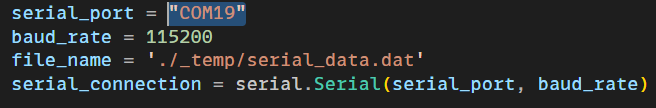
\includegraphics{figures/Script COM selection.png}
  \caption{Script USB Configuration}
  \end{figure}
 \item Run the script by typing: "python -u main.py" in the script fileLogger folder. 
\end{itemize}